\documentclass[twocolumn,superscriptaddress,showpacs,nofootinbib,notitlepage,preprintnumbers,secnumarabic,amssymb, floatfix, nobibnotes, aps, prd]{revtex4-2}
\usepackage[utf8]{inputenc}
\usepackage{graphicx}
\usepackage{latexsym,amsmath,amssymb,amsthm,lmodern,float,url}
\usepackage{natbib}
\usepackage{color}
\usepackage{microtype}
\usepackage{import}
\usepackage{bbold}
\usepackage[plain]{fancyref}
\usepackage{varioref}
\usepackage{subfigure}
\usepackage{soul}
\usepackage{slashed}
\usepackage{multirow}
\usepackage{lineno}
\usepackage{cancel}
\usepackage{tikz}
\usetikzlibrary{shapes}
\usetikzlibrary{positioning}
\usepackage[normalem]{ulem}
\usepackage{bbm}
\usepackage{qcircuit}
\usepackage[colorlinks=true,backref=false, linktocpage=true,
citecolor=blue,urlcolor=blue,linkcolor=blue,pdfpagemode=UseOutlines]{hyperref}
\hypersetup{%
  bookmarksnumbered=true,
  pdftitle = {},
  pdfsubject = {},
  pdfauthor = {},
  pdfkeywords = {}
}

\usepackage{orcidlink}

\newcommand{\ket}[1]{\left| #1 \right>} % for Dirac bras
\newcommand{\bra}[1]{\left< #1 \right|} % for Dirac kets
\newcommand{\braket}[2]{\left< #1 \vphantom{#2} \right|
 \left. #2 \vphantom{#1} \right>} % for Dirac brackets
\newcommand{\mbraket}[3]{\left< #1 \vphantom{#2#3} \right|
 #2 \left| #3 \vphantom{#1#2} \right>} % for Dirac matrix elements
%\newcommand{\mike}[1]{{\color{orange}Mike: #1}}
%\newcommand{\hank}[1]{{ \color{cyan}[{\bf Hank: #1}]\color{black}}}
%\newcommand{\ruth}[1]{{ \color{violet}[{\bf Ruth: #1}]\color{black}}}

\let\Re\undefined
\let\Im\undefined
\DeclareMathOperator{\Tr}{Tr}
\DeclareMathOperator{\Re}{Re}
\DeclareMathOperator{\Im}{Im}
\DeclareMathOperator{\tr}{Tr}
\DeclareMathOperator{\re}{Re}
\DeclareMathOperator{\im}{Im}

\usepackage{ninecolors}
\usepackage{relsize}
\newcommand\HS[1]{{\color{olive4}\smaller\textsf{[HS: #1]}}}

\newcommand{\inlinesection}[1]{\textbf{\emph{#1}}}
\newcommand{\CITEME}{{\color{red}~ CITEME}~}
\newcommand{\washington}{\texttt{ibm\_washington}}
\newcommand{\jakarta}{\texttt{ibmq\_jakarta}}
\newcommand{\nairobi}{\texttt{ibm\_nairobi}}
\newcommand{\manila}{\texttt{ibmq\_manila}}
\newcommand{\quito}{\texttt{ibmq\_quito}}

\newcommand{\fnal}{\affiliation{Fermi National Accelerator Laboratory, 
Batavia, IL 60510, USA}}

\linenumbers

\begin{document}
\preprint{FERMILAB-PUB-XX-XXX-T}
\title{Periodic Boundary Conditions for Lattice Field Theories with Circuit Knitting}

%%%% ADD YOURSELF TO AUTHOR LIST :D %%%%

\author{Gabrielle J. Bohner}
%\email{gbohner@fnal.gov}
\fnal

\author{Chantz A. Dalton}
%\email{cdalton@fnal.gov}
\fnal

\author{shabab m. kabir\,\orcidlink{0000-0002-9715-5249}}
% smk: my name is intentionally lowercase, thanks!
%\email{skabir@fnal.gov}
\fnal
\affiliation{Department of Physics, Grinnell College,
Grinnell, Iowa 50112, United States}

\author{Henry Lamm\,\orcidlink{0000-0003-3033-0791}}
\email{hlamm@fnal.gov}
\fnal

\author{Hersh Singh\,\orcidlink{0000-0002-2002-6959}}
\email{hershs@fnal.gov}
\fnal

\author{Peter Vander Griend}
%\email{peter.vandergriend@uky.edu}
\fnal
\affiliation{Department of Physics and Astronomy, University of Kentucky,
Lexington, Kentucky 40506, United States}


\author{Ruth S. Van de Water}
%\email{ruthv@fnal.gov}
\fnal

\author{Michael L. Wagman}
%\email{mwagman@fnal.gov}
\fnal

\begin{abstract}
Extracting physical point predictions from quantum simulations of lattice gauge theories requires treating the finite-volume corrections.  In this work, we investigate the cost associated with the approach to the infinite-volume limit with open and periodic boundary conditions.  While periodic boundary conditions have smaller finite-volume corrections, simulations with them require higher gate costs and connectivity. We further explore through numerical simulations the efficacy of circuit knitting to reduce these costs.
\end{abstract}

\maketitle

\section{Introduction}

Quantum simulation has the potential to become a powerful tool for investigating time-dependent phenomena in quantum field theories~\cite{Cloet:2019wre,Banuls:2019bmf,Bauer:2022hpo,Fang:2024ple}. Unlike classical computations, which quickly become intractable as system size grows, quantum computers are in principle well-suited to capture the full nonperturbative dynamics of these theories~\cite{Jordan:2011ne,Zohar:2012ay,Lamm:2019uyc,Ikeda:2020agk,Gustafson:2021imb,Cohen:2021imf,Barata:2022wim,Li:2022lyt,Carrillo:2024chu,Grieninger:2024axp,Barata:2024bzk,Farrell:2024fit,Li:2024nod,Farrell:2024mgu,Carena:2024peb,Chernyshev:2025lil,Shao:2025ygy,Andrade:2026lgt,Sukeno:2026mbqs}.

As with classical lattice field theory, quantum simulations require regulation.
Discretizing spacetime onto a lattice provides such a framework, but simulations at finite resources differ from the physical point. 
Systematic errors arise from sources including finite spatial volume, nonzero lattice spacing, digitization of the gauge field~\cite{Ciavarella:2025tdl}, approximating of the time-evolution operator~\cite{Kane:2025ybw}, and the use of unphysical masses. 
To make physical predictions, one must extrapolate results to the continuum, infinite-volume~\cite{Burbano:2025pef}, and physical-mass limits. 
The computational cost of a full simulation is, therefore, determined not only by the resources needed for an individual lattice but also by the ensemble of simulations required to perform these extrapolations.
In particular, the choice of boundary conditions affects the scaling in lattice length $L$ of extrapolation to the infinite-volume limit~\cite{Briceno:2020rar}, and on quantum computers, nonlocal operators may complicate this step~\cite{Briceno:2018lfj}.
Periodic boundary conditions (PBC) are typically preferred, as they preserve lattice translational invariance and thereby allow states to be classified by momentum. 
This property is especially useful for studying scattering and dynamical processes. 
There are, however, exceptions, for example in the study of topological observables, where open boundary conditions (OBC) may be more appropriate~\cite{Luscher:2011kk}.

From a hardware perspective, however, PBCs present a challenge. 
While they capture the desired physics, they introduce long-range interactions across the lattice. 
Quantum devices are generally restricted to one- or two-dimensional layouts with only local connectivity. 
Implementing periodicity, therefore, requires routing quantum information across the processor using a network of SWAP gates. 
The overhead from such SWAP networks can dominate the cost of a simulation~\cite{brierley2016efficientimplementationquantumcircuits,Zhu:2025upm,Parella-Dilme:2025yan} and can be particularly expensive when fermions are involved~\cite{PhysRevLett.120.110501}. 
For this reason, most quantum field theory simulations performed to date have adopted OBC, which, while incurring larger finite-volume corrections, avoid the nonlocality problem and are more amenable to current hardware constraints.

Recently, alternative strategies have been proposed to mitigate this difficulty. 
One such approach, known as circuit knitting~\cite{PhysRevLett.125.150504,Mitarai:2019vae,Piveteau:2021jup,Mitarai:2021sud}, replaces a single quantum circuit containing nonlocal entangling gates with an ensemble of circuits that involve only local gates and measurements. 
Classical post-processing is then used to reconstruct observables of the original circuit. 
In addition to reducing connectivity, the ``cutting'' of multi-qubit entangling gates , i.e., their replacement by multiple single-qubit gates, can lead to a reduction in errors~\cite{Yamamoto:2022yfd}. 
While circuit knitting can reduce quantum connectivity requirements, it introduces an exponential sampling and circuit-execution overhead in the number of cuts, together with additional classical reconstruction costs, and can suffer from degraded signal-to-noise ratios. 
Experimental demonstrations of circuit knitting have been performed~\cite{Singh:2023uhr}, and on-going research seeks to reduce the high costs and optimize cut placement~\cite{Perlin:2021,Chen:2022mgb,Lowe2023fastquantumcircuit,Lian:2023,Yang:2024jvu,10.1145/3579371.3589352,Piveteau:2025pso,Idan:2026cutting}.

In this work, we investigate the relative merits of three methods for approaching the infinite-volume limit in quantum simulations using {\color{red}\st{the} a} lattice $\mathbb{Z}_2$ gauge theory model as a test case: open boundary conditions, periodic boundary conditions implemented with SWAP networks, and periodic boundary conditions implemented with circuit knitting.

The remainder of this paper is organized as follows. 
In Sec.~\ref{sec:theory}, we review the lattice $\mathbb{Z}_2$ gauge theory with staggered matter, its Hamiltonian and the basic quantum circuits needed to simulate its time evolution.  
In Sec.~\ref{sec:infvolbc}, tensor network calculations are used to estimate the relative cost of reaching the infinite volume limit with OBC and PBC.  
Sec.~\ref{sec:knitting} discusses implementation of a virtual CNOT via circuit knitting with numerical results from \textsc{Qiskit} simulations presented in Sec.~\ref{sec:numresults}.  
Finally, we conclude and discuss future work in Sec.~\ref{sec:conclusion}.

\section{Theory}
\label{sec:theory}
\HS{Do we write the Gauss law somewhere?}
We begin by presenting the Hamiltonian describing $\mathbb{Z}_{2}$ lattice gauge theory in $1+1d$ with two-component Kogut-Susskind (staggered) fermions~\cite{PhysRevD.11.395,PhysRevD.13.1043}.
%\st{Here we investigate the $1+1d$ $\mathbb{Z}_2$ gauge theory using the Kogut-Susskind lattice Hamiltonian with two-component staggered fermionic matter and open and periodic boundary conditions -- OBCs and PBCs respectively}~\cite{PhysRevD.11.395,PhysRevD.13.1043}. }
In this model, all degrees of freedom have 2-state Hilbert space dimension which naturally maps to qubit-based quantum computers. 
We make no further simplifications to the Hilbert space as they do not persist in higher dimensions~\cite{Zohar:2021nyc}.  
For $N_{s}$ matter sites, the Hamiltonian is
% \begin{equation}
% \begin{split}
%     H =& \sum_{n=1}^{N_s - 1}\bigg[ \frac{1}{2 a_s}\sigma^{x}_{n,n+1} + \frac{a_s \eta }{2}(\bar{\psi}_n\sigma_{n,n+1}^{z}\psi_{n+1} + h.c.)\bigg]\nonumber\\
%     & +\ a_s m_0 \sum_{n=1}^{N_s}  (-1) ^{n}\bar{\psi}_n\psi_n,
% \end{split}
% \end{equation}
\begin{equation}
\begin{split}
    H =& \sum_{n=1}^{N}\bigg[ \frac{1}{2 a_s}\sigma^{x}_{n,n+1} + \frac{a_s \eta }{2}(\psi^{\dagger}_n\sigma_{n,n+1}^{z}\psi_{n+1} + h.c.)\bigg]\\
    & +\ a_s m_0 \sum_{n=1}^{N_s}  (-1) ^{n}\psi^{\dagger}_n\psi_n,
\end{split}
\end{equation}
where
\begin{equation}\label{eq:upper_limit}
    N = \left\{
    \begin{array}{l@{\,\,}l}
        N_{s} - 1 & \text{ OBC,} \\
        N_{s}     & \text{ PBC,}
    \end{array}
    \right.
\end{equation}
and 
\begin{equation}
    \psi_{N_{s}+1} \equiv \psi_{1},\quad \sigma^{i}_{N_{s}, N_{s}+1}\equiv \sigma^{i}_{N_{s},1}.
\end{equation}
The parameters $m_0$ and $\eta$ are the bare fermion mass and the gauge coupling respectively, $\psi_n$ is a fermion field on lattice site $n$, $\psi^{\dagger}_n$ is the corresponding antifermion field, and the Pauli matrices $\sigma_{n,n+1}^x$ and $\sigma_{n,n+1}^z$ act on the two-component state of the $\mathbb{Z}_2$ gauge-field, and $a_s$ is the spatial lattice spacing.   
The three terms in $H$ represent the gauge kinetic term, the fermion hopping term, and the fermion mass term, respectively. 
{\color{red}%\st{The difference between PBCs and OBCs comes from whether the  $\mathbb{Z}_2$ gauge-field can connect between the fermions at $n=N_s-1$ and $n=0$.}
Periodic boundary conditions are realized by implementing a gauge-field connection between the fermions at $n=N_{s}$ and $n=1$; open boundary conditions are realized by omitting such a connection.
In practice, this entails extending the upper limit of the sum over the gauge kinetic and fermion hopping terms to include a connnection between the terminal matter sites (cf. eq.~(\ref{eq:upper_limit}).} 
{\color{blue}(Does the following (correctly) address Hersh's comment?)}{\color{red}Alternatively, periodic boundary conditions can be implemented (following a Jordan-Wigner transformation) by means of a phase on the boundary site at {\color{blue}$n=N_{s}$}; we implement the connection explicitly as this procedure does not generalize to higher dimensions.}
\HS{if we don't have a $Z$ string for PBCs after Jordan-Wiger, then change discussion to say that we're hardcore bosons instead of fermions.}
\HS{I think I was talking about the $Z$ string from JW, not the gauge fields. It's correct that the Z string on the last link gets replaced a phase, which is the fermion parity. So we just need to include that in the last link after JW.}
For the remainder of the paper, we set $a_s = 1$ such that all dimensionful quantities are in lattice-spacing units.

\begin{figure*}[ht]
    \centering
    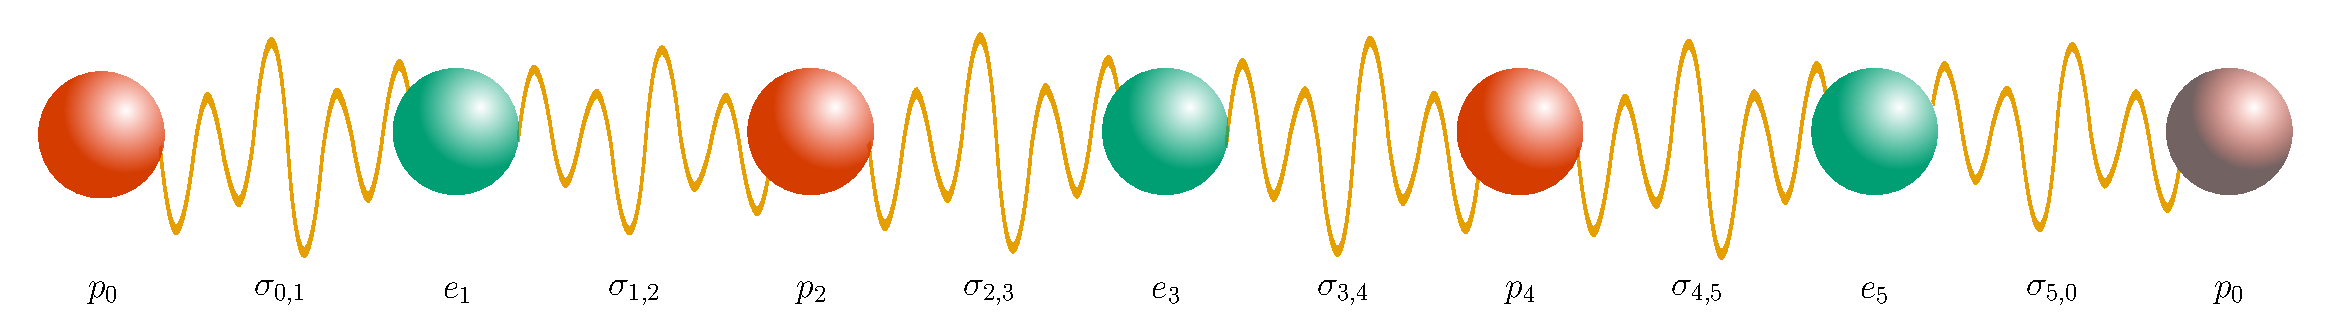
\includegraphics[width=\linewidth]{figures/lattice_z2_lbl.pdf}
    \caption{$N_s=6$ one-dimensional lattice used in this work. For PBCs (OBCs), the lattice is represented using twelve (eleven) qubits: three positron components $p_n$ on even sites colored, three electron components of the staggered fermion $e_n$ on odd sites colored green, and six (five) represent $\mathbb{Z}_2$-valued photon fields for which operators are labeled by adjacent pairs of lattice sites, e.g. $\sigma_{n,n+1}$ in orange.  The final positron is grayed to indicate the PBCs by using it as a shadow of $p_0$.} 
    \label{fig:schlat}
\end{figure*}

In the Kogut-Susskind fermion formulation, a single 2-component spinor $\psi(x)$ is described by two 1-component staggered fields $\psi_n$ on neighboring sites. 
Here, we denote the components on even sites by $p_n$ (for positron) and the components on odd sites by $e_n$ (for electron). 
A depiction for the case of $N_s=6$ is provided in Fig.~\ref{fig:schlat}. 
We perform a Jordan-Wigner transformation~\cite{JordanPWignerE} to convert the fermionic to bosonic degrees of freedom and write $H$ as
\begin{equation}
    \begin{split}
\label{eq:z2ham}
H = & \frac{1}{2} \sum_{n=0}^{N_s - 1} \sigma^{x}_{n,n+1} - \frac{m_0}{2} \sum_{n=0}^{N_s - 1} (-1)^n Z_{n}\\
&  + \frac{\eta}{4} \sum_{n=0}^{N_s-2}(X_n X_{n + 1} + Y_{n} Y_{n + 1})\sigma^{z}_{n,n+1},
\end{split}
\end{equation}
\HS{this is the place where we'd need include that extra parity phase in the last link for PBC.}
where the operators $X_n$, $Y_n$, and $Z_n$ denote Pauli matrices acting on the electron and positron qubit states.
%We note that for our model since the state of each degree of freedom can be encoded in a single qubit 
When we digitize the theory \HS{digitization isn't really needed, these are all qubits anyway.. so in a way digitization is trivial}, each site and link is represented by a single qubit; therefore, a lattice with $N_s$ sites can be encoded in $N_{q} = 2N_{s} -1$ qubits for OBC and $N_{q} = 2N_{s}$ qubits for PBC. %\st{$N_q = 2N_s - \delta_{OBC} $ qubits where $\delta_{OBC}$ indicates that when using OBCs there is one less photon gauge link.}}

\begin{figure*}[tb!]
    \centering
    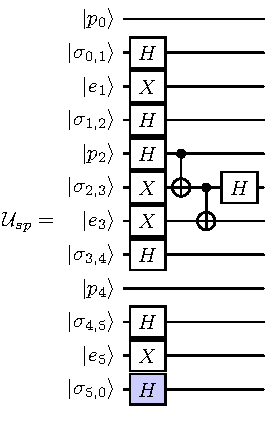
\includegraphics[width=0.28\linewidth]{figures/state_prep.pdf}\hspace{0.2cm}
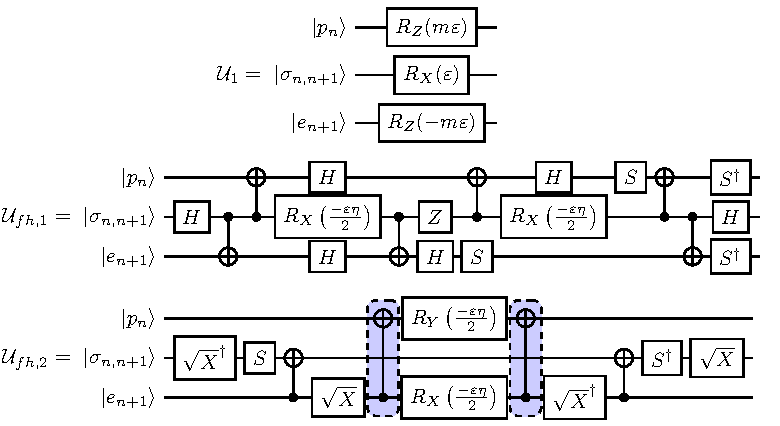
\includegraphics[width=0.69\linewidth]{figures/kinetics_hopping.pdf}
\caption{(left) Quantum circuit implementing initial-state preparation as $|\psi(6)\rangle = \mathcal{U}_{\text{sp}}|0....0\rangle$. We highlight the gate acting on the final qubit because it corresponds to the photon that only exists for PBC (right,top) The quantum circuit $\mathcal{U}_{1}$ implementing the gauge kinetic term and the fermion mass term (right,bottom) two equivalent quantum circuits implementing the fermion hopping term appearing in $\mathcal{U}_{2}$ and $\mathcal{U}_{3}$ are shown. These two circuits have different qubit connectivities and are used in conjunction to provide efficient mappings.  In $\mathcal{U}_3$ we highlight in blue the two CNOT gates that will be cut in the circuit knitting.
\label{fig:circs}
}
\end{figure*}

We approximate the time evolution operator $U(t)=e^{-iHt}$ via first order Trotterization~\cite{trotter1959product,Suzuki:1985,PhysRevX.11.011020} as,
\begin{equation}
    \label{eq:secondordertrotter}
    U(t) \approx \mathcal{U}(t/\varepsilon)^{N_t} ,
\end{equation}
where $N_t$ is an integer and $\epsilon \equiv t/N_t$.
To this end, we split the Hamiltonian of eq.~(\ref{eq:z2ham}) into a sum of three non-commuting operators
\begin{equation}
    H = \sum_{i=1}^3 H_i,
\end{equation} 
where 
\begin{equation}\label{eq:H2andH3}
\begin{split}
    H_1 &=  \frac{1}{2} \sum_{n=0}^{N_s - 1} \sigma^{x}_{n,n+1} - \frac{m_0}{2} \sum_{n=0}^{N_s - 1} (-1)^n Z_{n}, \\
    H_2 &=  \frac{\eta}{2} \sum_{n=\text{even}}^{N_s-2}(X_n X_{n + 1} + Y_{n} Y_{n + 1})\sigma^{z}_{n,n+1},\\
    H_3 &=  \frac{\eta}{2} \sum_{n=\text{odd}}^{N_s-2}(X_n X_{n + 1} + Y_{n} Y_{n + 1})\sigma^{z}_{n,n+1},
\end{split}
\end{equation}
where $H_1$ comprises the gauge-kinetic and fermion-mass terms and $H_2$ and $H_3$ are the even- and odd-site fermion-hopping terms, respectively {\color{red}(Peter: is there a factor of $2$ difference in the fermion hoppings terms between eqs.~(\ref{eq:z2ham}) and (\ref{eq:H2andH3})?)}. 
With these, the Trotterized time-evolution operator in Eq.~(\ref{eq:secondordertrotter}) is 
\begin{equation}
    \mathcal{U}(t/\varepsilon) = \prod_{i=1}^3 \mathcal{U}_i(t/\varepsilon)=\prod_{i=1}^3  e^{-i(t/\epsilon) H_i}.
\end{equation}


The implementation of these unitaries is shown in Fig.~\ref{fig:circs}. 
While $\mathcal{U}_1$ requires only single-qubit gates, $\mathcal{U}_{2}$ and $\mathcal{U}_{3}$ require entangling gates to implement the coupling between the fermionic sites.  
Because these are three-qubit gates, there is some freedom in implementing the connectivity between them. 
In order to efficiently leverage all available hardware, two circuit representations of the hopping-term operator are considered: $\mathcal{U}_{fh,1}$ and $\mathcal{U}_{fh,2}$. 
For these, both the number of CNOT gates and which qubits must have connectivity differ. 
As we implement circuit knitting, it will be desirable to cut the periodic lattice at points that would use $U_{fh,2}$ as the three qubits can be divided by cutting only 2 CNOTs rather than 3.

To keep the Hamiltonian sparse, we do not project to the gauge-invariant sector of Hilbert space.  As a consequence, we must explicitly enforce gauge invariance during the construction of the initial state.
Here our initial state $\ket{\phi}$ is taken as a linear superposition of two gauge-invariant states: the non-interacting vacuum state $\ket{\Omega}$  and a state $\ket{P}$ that has significant overlap with excited states such as electron-positron bound states. The superposition of these two states is 
\begin{equation}
    \label{eq:initstate}
    \ket{\phi(N_s)} = \frac{1}{\sqrt{2}}\Big(|\Omega(N_s)\rangle + |P(N_s)\rangle\Big),
\end{equation}
The states $|\Omega(N_s)\rangle$ and $|P(N_s)\rangle$ are defined for lattices of size $N_s$ as
% \begin{equation}
%   \begin{split}
%     \label{eq:compstates}
%     &{\color{red}\cancel{|\Omega(N_s)\rangle = \left(\prod_{n=\text{even}}^{N_2-2\delta_{OBC}}H_{n,n+1}X_{n+1}\right)\ket{0}^{\otimes 2N_s-1},}} \\
%     &{\color{red}|\Omega(N_s)\rangle_{OBC} = \left(\prod_{n=\text{even}}^{N_{s}-2}H_{n,n+1}X_{n+1}\right)\ket{0}^{\otimes 2N_s-1},}\\
%     &{\color{red}|\Omega(N_s)\rangle_{PBC} = \left(\prod_{n=\text{even}}^{N_{s}}H_{n,n+1}X_{n+1}\right)\ket{0}^{\otimes 2N_s-1},}\\
%     &|P(N_s)\rangle = X_m\sigma_{m,m+1}X_{n+1}\ket{\Omega(N_s)}.
%   \end{split}
% \end{equation}
\begin{equation}
  \begin{split}
    \label{eq:compstates}
    % &{\color{red}\cancel{|\Omega(N_s)\rangle = \left(\prod_{n=\text{even}}^{N_2-2\delta_{OBC}}H_{n,n+1}X_{n+1}\right)\ket{0}^{\otimes 2N_s-1},}} \\
    |\Omega(N_s)\rangle &= \left(\prod_{n=\text{even}}^{N}H_{n,n+1}X_{n+1}\right)\ket{0}^{\otimes 2N_s-1},  \\
    |P(N_s)\rangle &= X_m\sigma_{m,m+1}X_{n+1}\ket{\Omega(N_s)}.
  \end{split}
\end{equation}
where
\begin{equation}
    N = \left\{
    \begin{array}{l@{\,,\,}l}
        N_{s} - 2 & \text{OBC} \\
        N_{s}     & \text{PBC}
    \end{array}
    \right.
\end{equation}
where $H$ is the Hadamard gate and $m=N_s/2-1$ is the center lattice site.
The circuit to build this state from the computational $|0....0\rangle$ state for $N_s=6$ is given in the left of Fig. \ref{fig:circs}.

In general, the object of interest in quantum simulations of LGTs are correlation functions 
\begin{equation}
  C(t) =  \langle\phi | U^\dagger(t) O U(t) | \phi \rangle=\langle 0|\phi \, U^\dagger(t) O U(t) \, \phi^\dagger | 0 \rangle. \label{eq:correlator}
\end{equation}
which describe the evolution of an initial state $\ket{\phi} \equiv \phi^\dagger \ket{0}$ and its interaction with a operator $O$. 
The spectral representation of $C(t)$ is obtained by inserting complete sets of energy eigenstates $\ket{E_n}$
\begin{equation}
  C(t) = \sum_{n,m} \braket{\phi}{E_m } \braket{ E_n }{ \phi } \mbraket{E_m}{O}{E_n} e^{-i(E_n - E_m)t}. \label{eq:spec}
\end{equation}
Measurements of $|C(t)|^2$ from quantum simulations can be fit to this oscillatory form in order to extract energy differences $E_n - E_m$~\cite{Charles:2023zbl} for use in scale setting~\cite{Carena:2021ltu,Clemente:2022cka,Crippa:2024cqr}. In this work, we compute correlation functions involving $\ket{\phi}$ and the operator
\begin{equation}
\label{eq:exciteoperator}
    O_{n} = \psi^{\dagger}_n\sigma^{z}_{n,n+1}\psi_{n+1} + \psi^{\dagger}_n \sigma^{z}_{n, n+1}\psi^\dagger_{n+1} + h.c.\,,
\end{equation}
which in the qubit basis takes the form:
\begin{equation}
  O_{n} = X_n \sigma^z_{n,n+1} X_{n+1}.
\end{equation}
Furthermore, using Eq.~\eqref{eq:compstates}, we have 
\begin{equation}
    \begin{pmatrix}
    \mbraket{ \Omega }{ O }{ \Omega }&\mbraket{ P }{ O }{ \Omega }\\
    \mbraket{ \Omega }{ O }{ P }&\mbraket{ P }{ O }{ P }\\
    \end{pmatrix}=\begin{pmatrix}
        0&1\\
        1&0\\
    \end{pmatrix},
\end{equation}
such that the value of $C(t=0)$ is
\begin{equation}
  \begin{split}
    C(0) &= \mbraket{ \phi(N_s) }{ O }{ \phi(N_s) } = 1.
  \end{split}
\end{equation}

Correlation functions $C(t)$ as defined as in Eq.~\eqref{eq:correlator} with $\ket{\phi}$ as the initial state have time-dependence generically given by Eq.~\eqref{eq:spec}. 
In the limit $t\rightarrow\infty$, their Fourier transforms {\color{red}\st{should}} sharply peak about $E_m-E_n$ values.
If $\ket{\Omega}$ and $\ket{P}$ each overlap predominantly with a single energy eigenstate with energy $E_{\Omega}$ and $E_P$, respectively, then the time-dependence of $C(t)$ reduces to  
\begin{equation}
\begin{split}
  C(t)&\approx \cos[(E_P-E_{\Omega})t] \mbraket{\Omega}{O(t)}{P}\\
  &\hspace{10pt} + \frac{1}{2} \mbraket{\Omega}{O(t)}{\Omega} + \frac{1}{2} \mbraket{P}{O(t)}{P} \\
  &=\cos(M t)+\hdots \label{eq:spec01}
\end{split}
\end{equation}
where $M=E_P-E_{\Omega}$ is the energy difference between the eigenstates dominantly overlapping with $\ket{P(N_s)}$ and $\ket{\Omega(N_s)}$ and the ellipsis denotes contributions from other states with different $t$-dependence. 
Fits to Eq.~\eqref{eq:spec01} can interrogate this approximation.
If the single-state contribution $\cos(Mt)$ provides a good fit to $C(t)$, then $M$ can be expected to describe the energy gap between an electron-positron bound state and the vacuum, which corresponds to the mass of the particle associated with this state in the continuum and infinite-volume limits.
Finally, due to Trotterization, we do not obtain $C(t)$ from the quantum simulations but instead an approximation thereof defined as
\begin{equation}
    \label{eq:simobservable}
    \mathfrak{C}(t/\varepsilon) = \mbraket{ \phi(N_s) }{ \mathcal{U}^{\dagger}(t/\varepsilon)^{N_t} \ O \  \mathcal{U}(t/\varepsilon)^{N_t} }{ \phi(N_s) },
\end{equation}
where $\mathcal{U}(t/\varepsilon)$ is defined in Eq.~\eqref{eq:secondordertrotter}.  From this, the continuous time or continuum limit must be taken~\cite{Carena:2021ltu}.

\section{Infinite Volume Limit and Boundary Conditions}
\label{sec:infvolbc}

Quantum simulations will for some time be restricted to lattices with few sites.
How quickly an observable approaches its infinite-volume value as the lattice grows therefore decides how large a lattice is needed for a given accuracy, and the answer depends on the boundary conditions.
With PBC every site is equivalent, and in a theory with a mass gap the finite-volume corrections to single-particle masses fall off exponentially in the box length $L$ measured in units of the correlation length~\cite{Luscher:1985dn,Luscher:1986pf}.
With OBC the two ends of the lattice break translation invariance.
The ground state is distorted within a correlation length of each end, and a quantity averaged over the volume receives from these two boundary layers a correction proportional to the fraction of the volume they occupy, that is, to $1/L$~\cite{Symanzik:1981wd}.
Power-law rather than exponential finite-size corrections also arise, for different reasons, in chiral perturbation theory at small $m_\pi L$~\cite{Hasenfratz:1989pk} and in systems at criticality~\cite{Cardy:1984bb}.
In this section we first quantify both behaviors for the model of Sec.~\ref{sec:theory} with tensor-network calculations, and then estimate the gate cost of implementing PBC with SWAP networks.
In one dimension the box length in lattice units is the number of sites, $L=N_s$; we write $N_s$ in Sec.~\ref{sec:mass_gap_L} and keep $L$ for the discussion of general dimension in Sec.~\ref{sec:swap}.

\subsection{Finite-volume dependence of the meson gap}
\label{sec:mass_gap_L}

The electron-positron bound state of Sec.~\ref{sec:theory}, which we call the meson, is created from the vacuum by the operator $O_n$ of Eq.~\eqref{eq:exciteoperator}.
We ask how far its energy gap, measured with a volume-averaged operator on $N_s$ sites, lies from the infinite-volume value for each boundary condition.
All results are for $m_0=0.1$ and $\eta=0.5$, with matter sites labeled $n=1,\dots,N_s$ and the sums over links in Eq.~\eqref{eq:z2ham} running over the $N$ links of Eq.~\eqref{eq:upper_limit}.
Technical details are collected in App.~\ref{app:dmrg}.

The Hamiltonian commutes with the Gauss-law operators
\begin{equation}
\label{eq:gauss}
    G_n = \sigma^{x}_{n-1,n}\, Z_n\, \sigma^{x}_{n,n+1},
\end{equation}
and physical states, those without static charges, satisfy $G_n\ket{\psi}=(-1)^n\ket{\psi}$ for every $n$.
Time evolution preserves this condition, but a calculation of the spectrum encounters every sector.
We therefore add to $H$ the penalty $H_G=\tfrac{\lambda_G}{2}\sum_n[1-(-1)^nG_n]$ with $\lambda_G=20$, which vanishes on physical states and lifts all others far above the energies of interest.
With OBC the chain ends on matter sites, and the Gauss-law operator at each end needs a value for the electric field on the missing link, which is equivalent to placing a static charge beyond that end.
We choose the value for which no flux enters the chain; it is the choice whose spectrum corresponds to that of the periodic lattice.

An open chain has no momentum eigenstates, so we use an operator that is defined in the same way for both boundary conditions,
\begin{equation}
\label{eq:Odef}
   \mathcal{O} \equiv \frac{1}{\sqrt{N}} \sum_{n=1}^{N} O_n,
   \qquad
   O_n = X_n\,\sigma^{z}_{n,n+1}\,X_{n+1},
\end{equation}
which for PBC is the projection of $O_n$ onto zero momentum.
Let $\ket{E_j}$, $j=0,1,2,\dots$, be the eigenstates of $H+H_G$ in order of increasing energy; the ground state $\ket{E_0}$ is the interacting vacuum, not the product state $\ket{\Omega}$ of Eq.~\eqref{eq:compstates}.
The operator $\mathcal{O}$ connects the ground state to $\ket{E_j}$ with weight $w_j$ at the gap $\Delta_j$,
\begin{equation}
\label{eq:weights}
   w_j = \big|\mbraket{E_j}{\mathcal{O}}{E_0}\big|^2,
   \qquad
   \Delta_j = E_j-E_0 ,
\end{equation}
which are the weights and frequencies of the ground-state correlation function, $\mbraket{E_0}{\mathcal{O}(t)\,\mathcal{O}(0)}{E_0}=\sum_j w_j\,e^{-i\Delta_j t}$.
Such overlap factors also enter the extraction of matrix elements.

The lowest excitations form a band of single-meson states, $N_s$ of them for PBC and $N_s-1$ for OBC, with gaps between $1.287$ and $1.466$; the next levels begin near $2.34$.
With PBC, translation invariance lets $\mathcal{O}$ excite only the zero-momentum state, which is the highest of the band.
With OBC, $\mathcal{O}$ excites several states of the band, the highest carrying about $80\%$ of the weight, so no single eigenstate can be identified as the meson at rest.
We therefore use two moments of the weights over the band,
\begin{align}
\label{eq:Wdef}
   W &\equiv \sum_{j:\,\Delta_j<\Delta_{\rm cut}} w_j ,\\
\label{eq:Dbardef}
   \overline{\Delta} &\equiv \frac{1}{W}\sum_{j:\,\Delta_j<\Delta_{\rm cut}} w_j\,\Delta_j ,
\end{align}
with $\Delta_{\rm cut}=2$.
With PBC the weighted gap $\overline{\Delta}$ is the gap of the zero-momentum meson, which we call the meson gap, and the summed weight $W$ is the squared overlap of that state with $\mathcal{O}\ket{E_0}$.
At infinite volume each moment must take the same value for the two boundary conditions.
We take $\overline{\Delta}$ as the primary observable: it is an energy, like the quantity extracted in Sec.~\ref{sec:numresults}, and it does not depend on the normalization of $\mathcal{O}$.
The summed weight does: writing $N_s$ for $N$ in Eq.~\eqref{eq:Odef} changes the size and the sign of its $1/N_s$ correction for OBC, though not the fact that there is one.
We report $W$ as well because it is determined far more precisely.

We compute the lowest eigenstates of $H+H_G$ with the density-matrix renormalization group (DMRG)~\cite{White:1992zz} for even $N_s$ from $4$ to $18$ and for $N_s=24$.
The results agree with exact diagonalization at $N_s=4$ and $6$ to better than $4\times10^{-7}$, and two independent implementations agree to $3\times10^{-6}$ for $N_s\le10$.
The uncertainties are conservative estimates of the convergence error, not statistical standard deviations.

Figure~\ref{fig:fv_gaplo} shows both moments.
With PBC the weighted gap is $1.46407$ at $N_s=4$, $1.46643$ at $N_s=6$, and $1.46646$ at $N_s=8$ and $10$: it is $0.16\%$ below its limit at $N_s=4$ and within $0.002\%$ of it by $N_s=6$, as expected for exponentially small corrections.
The summed weight behaves in the same way.
We take the PBC values at $N_s=10$ as the infinite-volume results,
\begin{equation}
\label{eq:pbcinf}
   \overline{\Delta}_\infty = 1.46646(14), \qquad W_\infty = 0.6652838(4).
\end{equation}
With OBC the approach to the limit is slow.
The weighted gap is $3.6\%$ below $\overline{\Delta}_\infty$ at $N_s=4$ and still $0.5\%$ below at $N_s=24$, while the summed weight falls from $8.0\%$ above $W_\infty$ to $1.0\%$ above.

\begin{figure}[t]
    \centering
    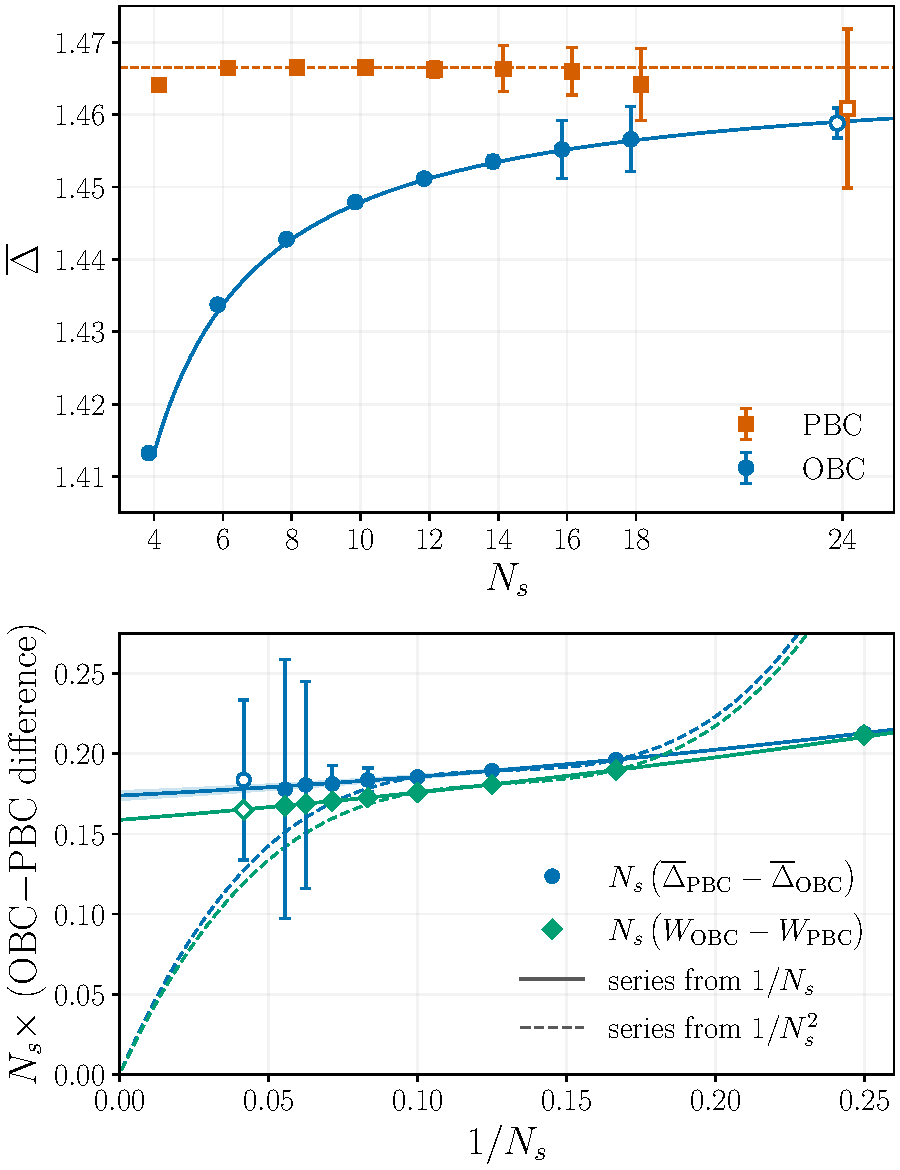
\includegraphics[width=\linewidth]{figures/fv_gaplo.pdf}
    \caption{Weighted gap $\overline{\Delta}$ (top) and summed weight $W$ (middle) versus $1/N_s$ for PBC (squares) and OBC (circles); $N_s$ is marked along the top.
    Dashed lines are the infinite-volume values of Eq.~\eqref{eq:pbcinf}, and solid curves are the fits of Eqs.~\eqref{eq:dbarfit} and~\eqref{eq:wfit}.
    Bottom: $N_s\,|y_{\rm OBC}-y_\infty|$ for $\overline{\Delta}$ (triangles) and $W$ (diamonds).
    Bands show the spread among acceptable fits (App.~\ref{app:dmrg}), and open symbols are not used in the fit shown.
    \label{fig:fv_gaplo}}
\end{figure}

The boundary-layer argument at the start of this section predicts that the OBC results approach the PBC limit as a power series in $1/N_s$ that begins at first order,
\begin{equation}
\label{eq:series}
   y_{\rm OBC}(N_s) = y_\infty + \frac{b}{N_s}+\frac{c}{N_s^2}+\frac{d}{N_s^3}+\dots ,
\end{equation}
where $y$ stands for $\overline{\Delta}$ or $W$.
We test this against corrections that fall off faster: a series that begins at $1/N_s^2$, as for a single energy level of a particle in a box; a single power $b/N_s^{\beta}$; and an exponential, with a free rate $\kappa$ or with the rate fixed to the meson gap, $M\equiv\overline{\Delta}_\infty$.
Each form is fitted to the OBC results for $N_{\min}\le N_s\le18$ with $y_\infty$ constrained to Eq.~\eqref{eq:pbcinf}, and $N_s=24$ is held out to test the prediction; the fits are listed in Table~\ref{tab:fv-fits} of App.~\ref{app:dmrg}.

For the summed weight the outcome is unambiguous.
The series of Eq.~\eqref{eq:series} through third order describes all sizes from $N_s=6$ and predicts $W=0.6721706(12)$ at $N_s=24$, where we measure $0.672161(11)$, while every alternative is rejected for all $N_{\min}\le10$.
For the weighted gap, whose uncertainties are larger, the same series describes all sizes from $N_s=4$ and no alternative does; some become acceptable once the smallest lattices are dropped.
The resulting fits are
\begin{align}
\label{eq:dbarfit}
   \overline{\Delta}_{\rm OBC}-\overline{\Delta}_\infty &= -\frac{0.174(3)}{N_s}-\frac{0.09(2)}{N_s^2}-\frac{0.26(5)}{N_s^3},\\
\label{eq:wfit}
   W_{\rm OBC}-W_\infty &= \frac{0.15876(6)}{N_s}+\frac{0.1464(9)}{N_s^2}\nonumber\\
   &\quad+\frac{0.243(3)}{N_s^3},
\end{align}
for $N_s\ge4$ and $N_s\ge6$, respectively.
Because the difference from the infinite-volume value falls as $1/N_s$, its product with $N_s$, shown in the bottom panel of Fig.~\ref{fig:fv_gaplo}, tends to $|b|$ rather than to zero.
If $y_\infty$ is left free in these fits, the OBC results alone give limits that differ from the PBC values by $+0.0004(16)$ for $\overline{\Delta}$ and $-0.00004(6)$ for $W$: the two boundary conditions agree at infinite volume to $0.1\%$ and $0.01\%$.
In practical terms, with OBC the weighted gap is within $1\%$ of its limit only for $N_s\ge14$, and $0.1\%$ would require $N_s\approx120$; with PBC it is within $0.16\%$ at $N_s=4$ and $0.002\%$ at $N_s=6$.

The $1/N_s$ correction has a simple origin: the operator $\mathcal{O}$ acts with the same amplitude on every link, but an open chain is distorted near its ends.
At $N_s=24$ the occupation of the matter sites in the ground state, $\nu_n\equiv\tfrac12\left[1-(-1)^n\langle Z_n\rangle\right]$, is $0.0635$ on every site with PBC; with OBC it is $0.0349$ on the end sites and returns to the PBC value within about three sites.
The terms of Eq.~\eqref{eq:Odef} inside these boundary layers are a fraction of order $1/N_s$ of the total, and they shift both moments by an amount of that order.
The same holds for any volume-averaged quantity; the mean occupation, for example, is lower with OBC by $0.052/N_s$.
Exponentially small corrections are negligible in comparison.

The $1/N_s$ correction is a property of volume-averaged quantities, not of every quantity on an open chain.
An individual level converges faster: the highest level of the OBC band lies below $\overline{\Delta}_\infty$ by about $0.39/N_s^2$ and is within $0.1\%$ of it for $N_s\ge18$.
Using that level requires resolving it from its neighbors, whose spacing also falls as $1/N_s^2$.
A correlation function of a volume-averaged operator followed for a shorter time oscillates at $\overline{\Delta}$, which carries the $1/N_s$ correction.

\subsection{SWAP cost}
\label{sec:swap}
Implementing the dynamics of a lattice gauge theory on a quantum processor requires either native connectivity between the qubits encoding interacting degrees of freedom or qubit routing.  
Fermionic-SWAP networks and their optimized variants for restricted hardware connectivity~\cite{Kivlichan:2017ngt,Hashim:2021loh}, together with general routing strategies for limited-connectivity devices~\cite{Cowtan:2019jqo}, provide the techniques applied to LGT routing.  
Here we first record the counts that follow from a direct embedding of a PBC LGT on a 2d square nearest-neighbor processor, with $\mathcal{F}$ the per-link overhead (physical qubits per logical site); these are to be read as upper bounds as more elaborate scheduling within the cited techniques can lower the prefactor without changing the $L$-scaling.  
This square-grid assumption is also relevant to IBM's Nighthawk generation, which uses degree-four square-lattice connectivity~\cite{ibm-processor-types}. 
By contrast, the Eagle-generation \washington{} model used in Sec.~\ref{sec:numresults} and the Heron r2/r3 processors use heavy-hex connectivity for which the finite-$L$ routing prefactor is architecture and compiler dependent.

For the 2d case with PBC mapped onto a 2d square processor, each of the
$L$ periodic links per direction requires $(L-1)$ SWAPs to bring
opposite-edge qubits adjacent.  Performing the routing in both spatial
directions and both senses (forward and back; the back sweep can in
principle be absorbed into the next Trotter step), the SWAP count per
Trotter step is
\begin{equation}
N_{\text{SWAP}}^{(2\text{d})} = 4L(L-1)\mathcal{F}.
\end{equation}
For a heavy-hex processor, the square-grid distance $L-1$ must be replaced by
graph distances in the chosen physical-qubit layout.  If
$\overline d_x(L)$ and $\overline d_y(L)$ are the average shortest-path
distances between the embedded qubits joined by periodic links in the two
directions, we define the following direct-routing {\color{red}\st{bookkeeping}} estimate {\color{red} \st{it} which} 
is not an optimized routing bound
\begin{equation}
N_{\text{SWAP}}^{(2\text{d},\,\mathrm{hh})}
\simeq 2L\left[\overline d_x(L)+\overline d_y(L)-2\right]\mathcal{F}
+N_{\mathrm{bulk}}^{(\mathrm{hh})}.
\end{equation}
The factor of $2$ accounts for forward and return routing.
$N_{\mathrm{bulk}}^{(\mathrm{hh})}$ denotes routing needed even away from the periodic boundary: the square-lattice interaction graph has degree-four vertices, whereas heavy-hex hardware has degree at most three and, therefore, does not natively embed every square-lattice nearest-neighbor interaction.
Square-lattice connectivity can nevertheless be emulated on heavy-hex with constant local routing overhead~\cite{ibm-heavy-hex}; comparative compilation studies likewise find topology-dependent communication overheads for heavy-hex and square processors~\cite{Rached:2024routing}.
For a local layout, $\overline d_{x,y}(L)=\mathcal{O}(L)$ and $N_{\mathrm{bulk}}^{(\mathrm{hh})}=\mathcal{O}(L^2\mathcal{F})$.  
Heavy-hex, therefore, preserves the $\mathcal{O}(L^2)$ scaling in 2d but generally changes the finite-size prefactor.  
In $1d$, a path can be embedded natively, so the leading distinction is instead the graph distance required to close the single periodic edge, as seen in the Washington compilation results of Table~\ref{tab:fig7-data}.

For the $3d$ case mapped onto the same 2d processor by laying the $L$ $2d$ layers side-by-side along one processor direction (each layer occupying an $L\!\times\!L$ patch), the per-step cost is the sum of $L$ copies of $N_{\text{SWAP}}^{(2\text{d})}$ plus an additional $2L^{2}(L-1)\mathcal{F}$ inter-layer SWAPs, 
\begin{equation}
    N_{\text{SWAP}}^{(3\text{d})} = 6L^{2}(L-1)\mathcal{F}.
\end{equation}
In general, a $d$-dimensional LGT mapped onto either local architecture in this way requires $\mathcal{O}(L^d)$ SWAP gates per Trotter step.  
The square and heavy-hex layouts share this volume scaling, while their coordination numbers, graph distances, and available embeddings determine different prefactors.  
Nighthawk's square lattice more closely realizes the assumptions behind the explicit counts above, while heavy-hex estimates should be obtained from a specified layout or transpilation rather than by assigning a universal replacement prefactor.

These estimates further assume nearest-neighbor interactions, an optimistic ansatz: improved LGT Hamiltonians~\cite{Carena:2022kpg,Gustafson:2023aai,Ciavarella:2023mfc,Illa:2025dou,Illa:2025njz} and domain-wall or overlap fermions for chiral gauge theories~\cite{Clancy:2023kla,Singh:2025sye,Lamm:2026qsp} both require beyond nearest-neighbor couplings.


\section{Basics of circuit knitting}
\label{sec:knitting}
Circuit knitting is a hybrid quantum–classical technique that enables non-local gates to be simulated by sampling a set of local
operations with a quasi-probability distribution~\cite{PhysRevLett.125.150504,Mitarai:2019vae,Piveteau:2021jup,Mitarai:2021sud}. Each subcircuit can be run independently on a quantum processor with reduced connectivity, and the results are then “knitted” back together using classical post-processing methods. The required operations are projective measurement of a qubit in Pauli basis, and single qubit rotations. The decomposition used here contains six terms per cut CNOT, producing $6^k$ subcircuits for $k$ independently cut CNOTs. Separately, the quasiprobability estimator has a sampling overhead of approximately $\mathcal{O}(9^k/\delta^2)$ to obtain an expectation value with statistical error $\delta$. {\color{red}(Peter: should we cite something for the scaling behavior?)}

{\color{magenta} Mike: yes! This is the most important number in the paper and if the answer is really that cost goes like $9^k$ in a stochastic version (if that's what that means..) aren't we making quantum simulation exponentially hard again? Only going a few number of trotter steps forever seems like a severe limitation, no?}

{\color{red}(Peter: this should be explained more/better)}
In Ref.~\cite{Mitarai:2019vae}, the decomposition of a CZ gate into single-qubit rotations and projective measurements is demonstrated. 
This result can be applied to the CNOT simply by applying two Hadamards. 
Alternatively, using the exponential form 
\begin{equation}
\begin{split}
    CNOT=&e^{i\frac{\pi}{4}(I-Z)(I-X)} \\
    =& e^{-i\frac{\pi}{4}(I\otimes X)}e^{-i\frac{\pi}{4}(Z\otimes I)}e^{i\frac{\pi}{4}(Z\otimes X)},
\end{split}
\end{equation}
one sees that the CNOT gate can be represented as two single-qubit rotations circuits and one multi-qubit gate. Following Fig. 2 in Ref.~\cite{Mitarai:2019vae}, this form can be represented as a sum of circuits seen in Fig.~\ref{fig:knitted_circuit}.
\begin{figure*}
    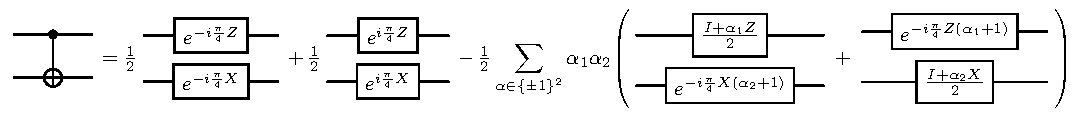
\includegraphics[width=\linewidth]{figures/cnot_circuit_knitting.pdf}
    \caption{Single-qubit decomposition of the CNOT gate.}
    \label{fig:knitted_circuit}
\end{figure*}

In practice, implementing these circuits then becomes a matter of straightforward book-keeping.  The first two terms, corresponding to unentangled pairs of single-qubit gates simply replace the CNOT in any circuit. For the projective measurements $\frac{I+\alpha_{1} Z}{2}$ and $\frac{I+\alpha_{2}X}{2}$, we perform a measurement in the correct basis, and add a count to the specific case. For example, for $\frac{I+\alpha_{1} Z}{2}$ we measuring either the $\ket{\uparrow}$ counts or $\ket{\downarrow}$ counts depending on the value of $\alpha_{1}$. $\frac{I+\alpha_{2}X}{2}$ is performed simply by applying a Hadamard gate to the second qubit and performing a measurement.

\section{Numerical Results}
\label{sec:numresults}
We anticipate the exponential growth in the number of circuits required as a function of ``cut'' CNOT gates will place sharp limits on maximum circuit depth for reasonable error.
We compute the mean fermion number and extract the mass parameter.
The mean fermion number oscillates sinusoidally about a decreasing value and with a decreasing amplitude.
We find this to be well approximated by a function of the form
\begin{equation}\label{eq:full_fit}
    \mathfrak{C}(t) = A\, e^{-B\,t}\, \cos{\left(C\,t\right)}+D+E\,t.
\end{equation}
The period of the oscillation is inversely proportional to the mass; see Fig.~\ref{fig:mass_scan}
In order to accurately extract the mass, we must probe as much of a complete oscillatory period as possible and anticipate needing at least a quarter of a cycle.
This implies the use of larger masses.
However, following the results of ref.~\cite{Charles:2023zbl} (see specifically table~III), we do not increase the mass arbitrarily high as this leads to a worse fit, as noted in the reference, perhaps due to couplings to other excited states.

\begin{figure}[ht]
    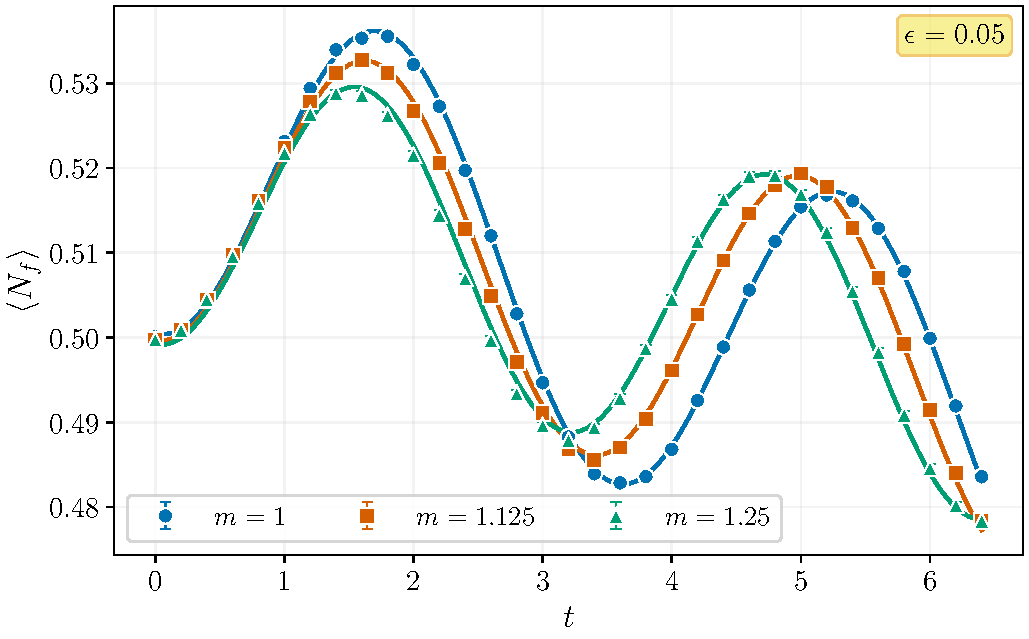
\includegraphics[width=0.48\textwidth]{figures/mass_scan.pdf}
    \caption{
    Mean fermion number from Trotter evolution time $t=0$ to $t=6.4$ for masses $m=1,\, 1.125,\ 1.25$ with a Trotter step of $\epsilon=0.05$.
    Points represent $N_{\mathrm{shots}}=1024^{2}$ with statistical errors smaller than marker size.
    Lines represent fits of points to Eq.~(\ref{eq:full_fit}).
    }
\label{fig:mass_scan}
\end{figure}

We proceed with $M=1.125$ and examine mass extractions for noiseless simulations.
Performing our circuit knitting procedure, we do not anticipate being able to access a third Trotter evolution step for reasonable time and computational resources.
We thus measure mean fermion number of the initial state at time $t=0$ with zero Trotter evolution steps; at times $t=0.2,\,0.4,\,0.6,\,0.8$ with one Trotter step; and at times $t=1,\,1.2,\,1.4,\,1.6$ with two Trotter steps.
As we here do not probe multiple periods of the evolution, we fit to a simplified functional form given by
\begin{equation}\label{eq:trunc_fit}
    \mathfrak{C}(t) = A \, \cos{\left(C\, t\right)} + D.
\end{equation}
We display the results in Fig.~\ref{fig:trotter_vs_exact} and summarize the extraction of the mass parameter $C$ in table~\ref{tab:mass_extraction}.
\begin{figure}[ht]
    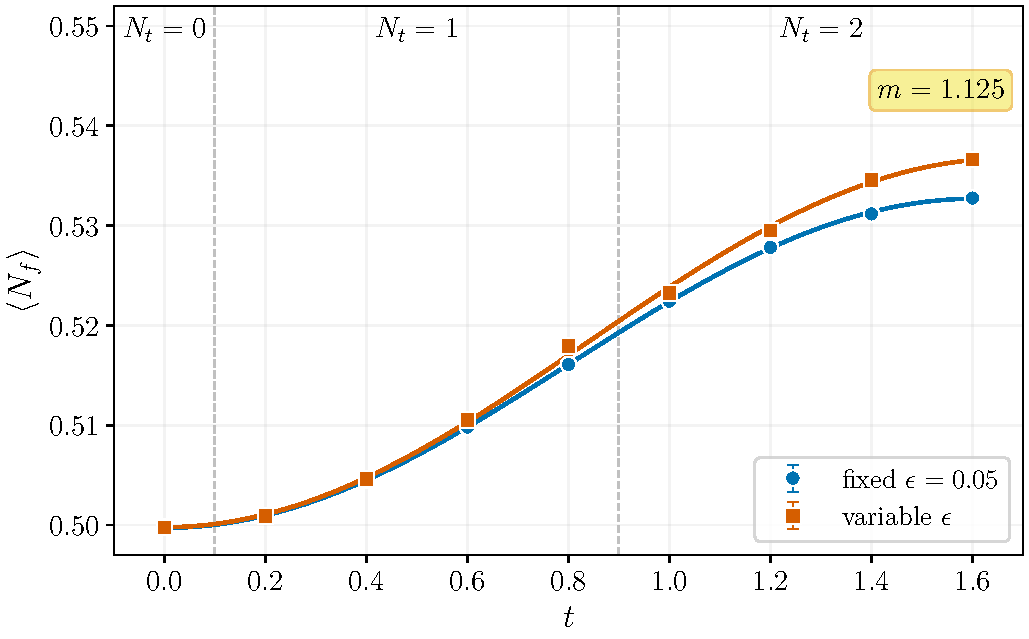
\includegraphics[width=0.48\textwidth]{figures/trotter_vs_exact.pdf}
    \caption{
    Mean fermion number from Trotter evolution time $t=0$ to $t=1.6$.
    Blue circles show the fixed-$\epsilon$ data and orange squares show the variable-step data.
    Points represent $N_{\mathrm{shots}}=1024^{2}$ with statistical errors smaller than marker size.
    Soft dashed lines separate the regions with zero, one, and two Trotter steps, labeled by $N_t$.
    Lines represent fits to Eq.~(\ref{eq:trunc_fit}).
    }
\label{fig:trotter_vs_exact}
\end{figure}

\begin{table}[t!]
\centering
    \begin{tabular}{ccc|c}\hline\hline
        points & fit & $\epsilon$ & $C$ \\ \hline
        33 & full & 0.05 & 1.87 \\
        9 & trunc. & 0.05 & 1.96 \\
        9 &  trunc. & var. & 1.88 \\
        9 & trunc. & 0.025 & 1.95 \\
        \hline\hline
    \end{tabular}
\caption{
   Mass parameter extraction for $M=1.125$.
   $33$ points corresponds to fitting multiple oscillatory periods from time $t=0$ to $t=6.4$; 9 points corresponds to fitting from time $t=0$ to $t=1.6$.
   Full fit corresponds to the oscillatory Ansatz of Eq.~(\ref{eq:full_fit}) while truncated (``trunc.'') fit corresponds to that of Eq.~(\ref{eq:trunc_fit}).
   Variable (``var.'') step size varying the Trotter step size between 0.2 and 0.8 for 1 or two steps as described in the text.
}
\label{tab:mass_extraction}
\end{table}

\subsection{Noisy circuit-knitting comparison}

All noisy results in this subsection are local simulations using the noise
properties and device topology encoded in
\textsc{Qiskit's} \texttt{FakeWashingtonV2} representation of the 127-qubit
\washington{} backend.  Circuits were transpiled at optimization level one
against the same backend model.  Thus ``noisy'' refers to simulation with the
Washington calibration-derived device model, not execution on the physical
device.

The \washington{} calibration is an Eagle r1-era benchmark and should not be
interpreted as the absolute noise level of current IBM hardware.  Washington
contained 127 qubits on a heavy-hex lattice.  Heron r1 increased this to 133
qubits, and Heron r2/r3 to 156 qubits, while retaining heavy-hex connectivity
and introducing fixed-frequency qubits with tunable
couplers~\cite{ibm-processor-types}.  IBM reported a
three- to five-fold device-performance improvement for Heron r1 over its
flagship Eagle processors, largely through improved two-qubit control and
suppressed crosstalk~\cite{ibm-heron-system-two}; a late-2025 Heron r3 system
reported a best error per layered gate (EPLG) of approximately
$0.23\%$~\cite{ibm-q4-2025}.  The Washington model therefore remains useful
for a controlled comparison of knitting with and without a heavy-hex routing
constraint, but likely overstates the absolute noise expected from current
Heron hardware.  Nighthawk changes the connectivity comparison more
fundamentally: its degree-four square lattice is closer to the architecture
assumed in Sec.~\ref{sec:swap} and should reduce routing relative to heavy-hex,
potentially decreasing the hardware-level advantage obtained by cutting a
periodic edge~\cite{ibm-processor-types}.

% \begin{figure}
%     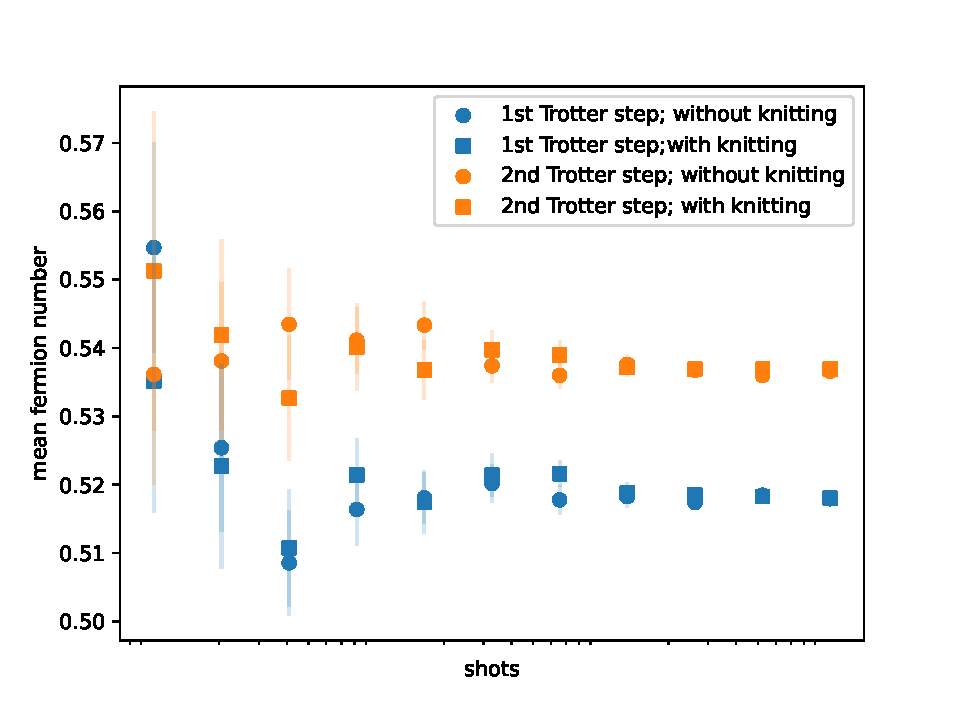
\includegraphics[width=0.48\textwidth]{figures/noiseless_convergence.pdf}
%     \caption{
%         Plot of the mean fermion number for 1 and 2 Trotter evolution steps (blue and orange points, respectively) in a noiseless simulation with a spacing of $\epsilon=0.8$.
%         We observe the knitted results (square markers) to converge to the non-knitted results (circular markers) as the number of shots is increased.
%         The number of shots displayed on the x-axis is normalized to emphasize convergence.
%         Error bars represent statistical uncertainties.
%     }
% \label{fig:noisy_convergence}
% \end{figure}

% \begin{figure}
%     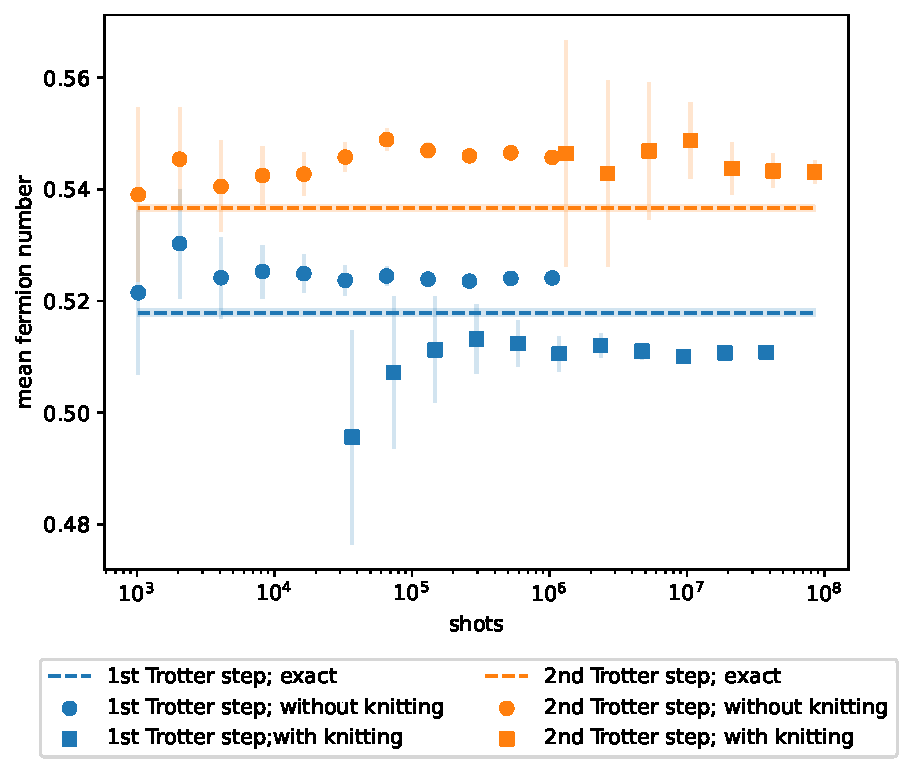
\includegraphics[width=0.48\textwidth]{figures/noisy_convergence.pdf}
%     \caption{
%         Plot of the mean fermion number for 1 and 2 Trotter evolution steps (blue and orange points, respectively) in a noisy simulation with a spacing of $\epsilon=0.8$.
%         We observe that in the presence of noise neither the non-knitted results (circular markers) nor the knitted results (square markers) converge to the exact results (dotted lines and error bands taken from the highest statistics non-knitted points of Fig.~\ref{fig:noisy_convergence}).
%     }
% \end{figure}

\begin{figure*}
    \centering
    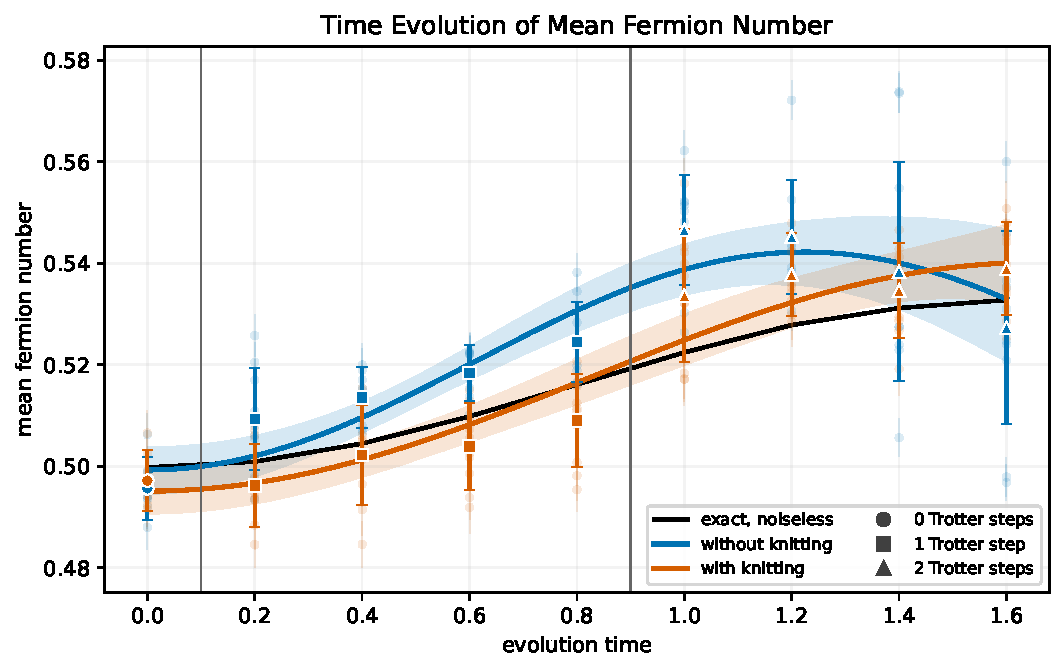
\includegraphics[width=0.98\textwidth]{figures/fermion_number_with_vs_without_knitting_scatter.pdf}
    \caption{Time evolution of the mean fermion number without (blue) and
    with (orange) circuit knitting.  Points and error bars are the resampled
    central values and one-standard-deviation uncertainties; circles denote
    results without knitting and squares denote results with knitting. Soft dashed lines
    separate the regions with zero, one, and two Trotter steps, labeled by $N_t$. The
    black curve is the noiseless fixed-step result at $\epsilon=0.05$.  Colored curves and bands show
    the primary weighted fits and their 68\% parametric-bootstrap intervals. {\color{magenta} Mike: explain resampling details, is this empirical bootstrap intervals after some sampling definition}}
    \label{fig:knitting-time-evolution}
\end{figure*}

% Generated by scripts/fit_fig7.py; do not edit by hand.
\begin{table}[t!]
\centering
\small
\begin{tabular}{c|c|c|c|c|c|c|c}\hline\hline
\multirow{2}{*}{$t$} & \multirow{2}{*}{$N_t$} & \multirow{2}{*}{$k$}
& terms
& \multicolumn{2}{c|}{$N_{\mathrm{CNOT}}$}
& \multicolumn{2}{c}{$\langle N_f\rangle$} \\ \cline{5-8}
& & & $(6^k)$ & no knit & knit & no knit & knit \\ \hline
$0.0$ & 0 & 0 & 1 & $2$ & $2$ & $0.496(6)$ & $0.497(6)$ \\ \hline
$0.2$ & \multirow{4}{*}{1} & \multirow{4}{*}{2} & \multirow{4}{*}{36} & \multirow{4}{*}{$41\text{--}50$} & \multirow{4}{*}{$39$} & $0.509(10)$ & $0.496(8)$ \\
$0.4$ &  &  &  &  &  & $0.514(6)$ & $0.50(1)$ \\
$0.6$ &  &  &  &  &  & $0.518(5)$ & $0.504(9)$ \\
$0.8$ &  &  &  &  &  & $0.524(8)$ & $0.509(9)$ \\ \hline
$1.0$ & \multirow{4}{*}{2} & \multirow{4}{*}{4} & \multirow{4}{*}{1{,}296} & \multirow{4}{*}{$98\text{--}116$} & \multirow{4}{*}{$67\text{--}85$} & $0.547(11)$ & $0.534(13)$ \\
$1.2$ &  &  &  &  &  & $0.545(11)$ & $0.538(8)$ \\
$1.4$ &  &  &  &  &  & $0.54(2)$ & $0.535(9)$ \\
$1.6$ &  &  &  &  &  & $0.527(19)$ & $0.539(9)$ \\
\hline\hline
\end{tabular}
\caption{Noisy data plotted in Fig.~\ref{fig:knitting-time-evolution} and the
associated sampling cost.  Each direct circuit and each knitted decomposition
term used $2^{14}=16{,}384$ shots for each of ten independent seeds.  The
aggregate count for each knitted data point is therefore
$N_{\mathrm{shots}}=(6^k)\mathbin{\times}10\mathbin{\times}2^{14}$; each
no-knit point has $N_{\mathrm{shots}}=10\mathbin{\times}2^{14}$.  Here
$k$ counts only the CNOTs replaced by circuit cuts, not all CNOTs in the
transpiled circuits.  The $N_{\mathrm{CNOT}}$ entries give compiled CNOT
counts observed in a compilation-only reconstruction with
\texttt{FakeWashingtonV2}, optimization level one, and eleven transpiler
seeds.  The two-layer knitted range samples six representative decomposition
terms per seed and is not retained metadata from the original runs.
Uncertainties are the one-standard-deviation resampling
uncertainties used in Fig.~\ref{fig:knitting-time-evolution}.}
\label{tab:fig7-data}
\end{table}


The compiled CNOT counts in Table~\ref{tab:fig7-data} also quantify the
routing benefit of cutting the periodic link on the Washington heavy-hex
topology.  For the fixed transpiler seed used in our reproducible reference
compilation, the one-step circuit decreases from 50 CNOTs without knitting to
39 CNOTs per knitted term, a 22\% reduction.  Only two of the eleven removed
CNOTs are the explicitly cut gates; the other nine arise from avoided
routing.  At two steps the corresponding counts are 104 and 76, a 27\%
reduction, of which four are cut gates and 24 are avoided routing CNOTs.  The
absolute routing saving therefore grows approximately with $N_t$, although
the ranges in Table~\ref{tab:fig7-data} show that its precise value depends on
the transpiler layout and seed.  These Washington-specific compiled counts
are distinct from the idealized square-lattice SWAP-network estimates in
Sec.~\ref{sec:swap}.

Fig.~\ref{fig:knitting-time-evolution} compares the noisy simulations with
and without circuit knitting against a noiseless fixed-step reference at
$\epsilon=0.05$.  This reference is itself a finite-Trotter, finite-shot
simulation rather than exact Hamiltonian evolution.  The fitted colored data
add the device-derived noise model and finite-shot fluctuations.
If noisy CNOTs dominate the uncertainty, the smaller CNOT count in each
knitted term should reduce the device-noise contribution to the scatter and
can therefore narrow the associated error bars.  This benefit competes with
the variance amplification of the quasiprobability reconstruction and its
finite sampling.  Consequently, fewer compiled CNOTs do not by themselves
guarantee smaller total knitted error bars.

We fit the same nine time points in each series to both
Eqs.~(\ref{eq:trunc_fit}) and~(\ref{eq:full_fit}), using the resampling
uncertainties as independent absolute weights.  For the truncated model,
$A$ is the oscillation amplitude, $C$ is the frequency used as the effective
mass estimator, and $D$ is the mean offset over the fitted window.  Parameter
uncertainties and differences are obtained from 10,000 parametric-bootstrap
replicas, in which each time point is independently drawn from a Gaussian
with its measured central value and resampling uncertainty.  We also fit the
noiseless fixed-step reference only at these nine times so that comparisons
use the same limited temporal window rather than a more strongly constrained
long-time fit.

The five-parameter form is not supported by this short time range: it
has substantially larger AICc values than the truncated cosine and frequently
places at least one parameter on a fit boundary.  We therefore use the
truncated cosine as the primary model.  Table~\ref{tab:fig7-fits} reports all
three primary-fit parameters; the uncertainty on $C$ is emphasized because it
is the parameter relevant to the mass comparison.

% Generated by scripts/fit_fig7.py; do not edit by hand.
\begin{table*}[t!]
\centering
\begin{tabular}{lccccc}\hline\hline
data & $A$ & $C$ & $D$ & $\chi^2/\mathrm{dof}$ & AICc \\ \hline
noiseless, $\epsilon=0.05$ & $-0.0165^{+0.0002}_{-0.0002}$ & $1.96^{+0.03}_{-0.03}$ & $0.5162^{+0.0002}_{-0.0002}$ & 0.25/6 & 11.05 \\
noisy, without knitting & $-0.022^{+0.004}_{-0.005}$ & $2.6^{+0.3}_{-0.4}$ & $0.521^{+0.005}_{-0.004}$ & 2.70/6 & 13.50 \\
noisy, with knitting & $-0.024^{+0.005}_{-0.01}$ & $1.9^{+0.4}_{-0.6}$ & $0.519^{+0.011}_{-0.004}$ & 2.04/6 & 12.84 \\ \hline\hline
\end{tabular}
\caption{Weighted truncated cosine fits to the same nine time points shown in Fig.~\ref{fig:knitting-time-evolution}. Here $A$, $C$, and $D$ are the amplitude, frequency, and offset in Eq.~\eqref{eq:trunc_fit}. Each entry gives the bootstrap median and central 68\% parametric-bootstrap interval.}
\label{tab:fig7-fits}
\end{table*}

Using the model-selection rule described in the text, the truncated cosine is the
primary model.  The fitted knitted-minus-un-knitted frequency difference is
$\Delta C=-0.692^{+0.534}_{-0.647}$
(68\% parametric-bootstrap interval).


Relative to the matched noiseless fixed-step reference in
Table~\ref{tab:fig7-fits}, neither the knitted nor the un-knitted frequency
shift is resolved at 95\% confidence.

The knitted frequency interval is more asymmetric because the knitted data do
not show a clear turnover within the fitted time range and have larger
late-time uncertainties.  Bootstrap fluctuations can therefore place the
maximum beyond the final time point, producing a long low-frequency tail.  In
contrast, the un-knitted data turn over near $t\simeq1.2$, constraining both
sides of the frequency distribution.  Correspondingly, 4.61\% of the knitted
bootstrap fits approach a parameter bound, compared with 0.13\% without
knitting.  This asymmetry is induced by the short-window nonlinear fit, not by
asymmetric pointwise measurement errors.

The 95\% bootstrap interval for the frequency difference is
$-2.370 < \Delta C < 0.425$.  Thus the central values suggest a lower
frequency after knitting, but the present statistics do not resolve a
nonzero shift at 95\% confidence.

\section{Conclusions}
\label{sec:conclusion}

In this work we have investigated the interplay of finite-volume
systematics and gate costs in quantum simulations of lattice gauge
theories, using 1+1d $\mathbb{Z}_2$ with staggered matter as a
controlled test case.  Although OBC reduces the gate count at fixed
$L$ by eliminating the periodic link, the larger finite-volume errors
under OBC require correspondingly larger $L$ to reach a given target
precision --- gains from the cheaper gate count can therefore be wiped
out by the inflated volume.  We demonstrate this with tensor-network
calculations of the meson gap obtained from a volume-averaged operator.
With PBC the gap is within $0.002\%$ of its infinite-volume value at
$N_s=6$.  With OBC it approaches the same value only as $1/N_s$, so
that $0.1\%$ accuracy would require $N_s\approx120$; the
infinite-volume limits obtained with the two boundary conditions differ
by $0.0004(16)$, consistent with zero.
A direct PBC embedding via SWAP
networks, on the other hand, costs $4L(L{-}1)\mathcal{F}$ per Trotter
step in 2d and $6L^2(L{-}1)\mathcal{F}$ in 3d --- an $\mathcal{O}(L^d)$
overhead that grows rapidly with dimension.  Both observations make
the potentially exponential circuit-execution and sampling cost of circuit knitting
attractive in regimes where the cut count $k$ remains modest.

To probe the realistic cost-vs-fidelity tradeoff of circuit knitting in
this setting, we performed both noiseless and noisy \textsc{Qiskit}
simulations at $L=4$, cutting the two CNOTs that close the periodic
boundary in $\mathcal{U}_3$.  The knitted circuits reproduce the
mean-fermion-number evolution through two full Trotter steps using
$N_{\mathrm{shots}}=16{,}384$ per sub-circuit for each of ten seeds.  The primary noisy-data fits give a
knitted-minus-un-knitted frequency difference whose 95\% bootstrap interval
includes zero (Tab.~\ref{tab:fig7-fits}); the current statistics therefore do
not resolve a knitting-induced shift.  In our exhaustive implementation,
$k$ cut CNOTs produce $6^k$ decomposition terms.  At fixed shots per term,
this growth ruled out a third Trotter step within our computational budget:
three layers require $k=6$, corresponding to $6^6=46{,}656$ subcircuits per
seed.  More generally, maintaining a fixed statistical precision $\delta$
incurs a quasiprobability sampling overhead of approximately
$\mathcal{O}(9^k/\delta^2)$.  This exponential growth is the dominant practical
bottleneck of the technique --- its mitigation is therefore a
prerequisite for scaling these studies to larger systems.  The recent
integration of circuit knitting into the \textsc{Qiskit} addon
framework~\cite{qiskit-addon-cutting} will streamline such extensions
at the engineering level.

Several directions merit further study.  The cost comparison
generalizes naturally to higher-dimensional gauge theories --- first
to 2+1d and 3+1d $\mathbb{Z}_2$, then to the non-abelian SU(2) and
SU(3) cases relevant to QCD --- where the $\mathcal{O}(L^d)$ SWAP
scaling makes the knitted alternative increasingly attractive but the
per-cut sampling cost grows in concert.  Reducing this sampling
overhead is the central open problem.  Joint-cut decompositions for
multiple two-qubit gates strictly outperform $k$ independent
cuts~\cite{Schmitt:2023urx}, classical communication between
sub-circuits lowers the optimal asymptotic sampling overhead for $n$ parallel wire cuts from
$\mathcal{O}(16^n)$ to
$\mathcal{O}(4^n)$~\cite{Brenner:2023txj,Harada:2023yqg}, and
variational or Monte-Carlo-importance-sampled schemes co-optimize the
quasi-probability decomposition with the target observable to keep the
sampling cost under a user-chosen budget~\cite{Gentinetta:2023gne}.
Adapting these techniques to lattice-gauge-theory circuits is a
particularly promising direction, since lattice applications have been
largely absent from the circuit-knitting literature to date.
Extending the comparison to improved LGT
Hamiltonians~\cite{Carena:2022kpg,Gustafson:2023aai,Ciavarella:2023mfc,Illa:2025dou,Illa:2025njz}
and chiral lattice fermions~\cite{Clancy:2023kla,Singh:2025sye,Lamm:2026qsp}, both
of which require beyond-nearest-neighbor couplings, will sharpen the
cost-versus-fidelity tradeoffs we have identified here.

\begin{acknowledgments}
The authors acknowledge the support by the Department of Energy through the Fermilab QuantiSED program under the grant ``Toward Lattice QCD on Quantum Computers". This work was produced by Fermi Forward Discovery Group, LLC under Contract No. 89243024CSC000002 with the U.S. Department of Energy, Office of Science, Office of High Energy Physics. 
\end{acknowledgments}

\appendix

\section{Details of the tensor-network calculations}
\label{app:dmrg}

With OBC the end sites lack one link, and we write $G_1=q_L\,Z_1\,\sigma^{x}_{1,2}$ and $G_{N_s}=\sigma^{x}_{N_s-1,N_s}\,Z_{N_s}\,q_R$ with $q_L,q_R=\pm1$.
We use $q_L=q_R=-1$, the value that $\sigma^x$ takes on a link without flux.
Exact diagonalization at $N_s=4$ and $6$ confirms that the lowest excitation then lies $1.29$ above the ground state, as with PBC, whereas each end with $q=+1$ adds a state at $1.05$, bound to the static charge at that end.

The eigenstates of $H+H_G$ are computed as matrix product states with \textsc{ITensor}~\cite{Fishman:2020gel}, the excited states one after another by DMRG with an energy penalty for overlap with the states already found.
We compute the lowest $31$ states ($41$ for OBC at $N_s=16$ and for $N_s=24$), which contain the whole single-meson band at every size.
The truncation error per bond is $10^{-11}$, and the bond dimension of the converged states did not exceed $65$ wherever it was recorded, far below the cap of $300$ to $400$.
Each state receives between several hundred and several thousand sweeps, in successive stages for $N_s\ge14$, and results are averaged over up to four random starting states.

DMRG reproduces exact diagonalization at $N_s=4$ and $6$ to $4\times10^{-7}$ in both moments, and a second, independent implementation agrees to $3\times10^{-6}$ for $N_s\le10$.
The uncertainty on $\overline{\Delta}$ combines in quadrature three contributions: the energy standard deviation of each state, $(\langle (H+H_G)^2\rangle-\langle H+H_G\rangle^2)^{1/2}$, which bounds its distance from an exact eigenvalue~\cite{Weinstein:1934}, propagated through Eq.~\eqref{eq:Dbardef}; the scatter among starting states; and, for $N_s\ge14$, the change in the last stage of the calculation.
For PBC with $N_s\ge12$, where the answer is known from the smaller lattices, the actual deviations are at most half of this estimate and all negative: incomplete convergence lowers $\overline{\Delta}$.
The uncertainty on $W$ combines the scatter among starting states, the difference between the two implementations, and the change in the last stage.
The summed weight is far better determined than $\overline{\Delta}$ because it is unchanged when DMRG mixes neighboring levels of the band.
Table~\ref{tab:fv-data} lists both moments.

% Generated by finite_volume/fit_fv.py; do not edit by hand.
\begin{table*}[t]
\centering
\begin{tabular}{r@{\qquad}l@{\qquad}l@{\qquad}l@{\qquad}l}\hline\hline
$N_s$ & $\overline{\Delta}_{\rm PBC}$ & $\overline{\Delta}_{\rm OBC}$ & $W_{\rm PBC}$ & $W_{\rm OBC}$ \\ \hline
4 & 1.464073(10) & 1.41324018(45) & 0.66565392(33) & 0.71822633(33) \\
6 & 1.466430(24) & 1.4337440(89) & 0.66527338(33) & 0.69693544(33) \\
8 & 1.466463(89) & 1.442786(37) & 0.66528353(33) & 0.68789084(34) \\
10 & 1.46646(14) & 1.447912(62) & 0.66528378(33) & 0.68286684(34) \\
12 & 1.4663(11) & 1.45115(62) & 0.6652850(21) & 0.6796693(30) \\
14 & 1.4663(32) & 1.45352(81) & 0.6652833(76) & 0.6774565(66) \\
16 & 1.4660(33) & 1.4552(41) & 0.665267(24) & 0.675835(17) \\
18 & 1.4641(50) & 1.4566(45) & 0.6652760(55) & 0.674594(21) \\
24$^{*}$ & 1.461(11) & 1.4588(21) & 0.6652734(55) & 0.672161(11) \\
\hline\hline
\end{tabular}
\caption{Weighted gap $\overline{\Delta}$ and summed weight $W$ of the single-meson band, Eqs.~\eqref{eq:Wdef} and~\eqref{eq:Dbardef}, for periodic and open boundary conditions at $(m_0,\eta)=(0.1,0.5)$.  Uncertainties on $\overline{\Delta}$ are dominated by bounds from the energy variance of the DMRG states and by the change in the last refinement stage, and are not statistical; those on $W$ combine the scatter among starting states, the difference between the two implementations, and the change in the last refinement stage.  The starred size is not used in any fit.}
\label{tab:fv-data}
\end{table*}


In the fits, $y_\infty$ is a parameter constrained by Eq.~\eqref{eq:pbcinf}, which enters the $\chi^2$ as one additional data point, and a fit is acceptable if its $\chi^2$ probability exceeds $5\%$.
Table~\ref{tab:fv-fits} gives the results for each form.
Because the uncertainties on $\overline{\Delta}$ are conservative, acceptable fits to it have $\chi^2$ well below the number of degrees of freedom.
The fits of Eqs.~\eqref{eq:dbarfit} and~\eqref{eq:wfit} use the smallest possible $N_{\min}$ and then the lowest acceptable order.
Lowering the order or raising $N_{\min}$ among acceptable fits moves the leading coefficient within $-0.181$ to $-0.162$ for $\overline{\Delta}$ and $0.1566$ to $0.1589$ for $W$, the range shown by the bands in Fig.~\ref{fig:fv_gaplo}.

% Generated by finite_volume/fit_fv.py; do not edit by hand.
\begin{table*}[t]
\centering
\begin{tabular}{l|cccc|cccc}\hline\hline
 & \multicolumn{4}{c|}{$\overline{\Delta}$} & \multicolumn{4}{c}{$W$} \\
 & $N_{\min}=4$ & $N_{\min}=6$ & & at $N_s=24$ & $N_{\min}=4$ & $N_{\min}=6$ & & at $N_s=24$ \\
$y_{\rm OBC}(N_s)-y_{\infty}$ & $\chi^2/{\rm dof}$ & $\chi^2/{\rm dof}$ & $N_{\min}^{\rm acc}$ & pull & $\chi^2/{\rm dof}$ & $\chi^2/{\rm dof}$ & $N_{\min}^{\rm acc}$ & pull \\ \hline
$b/N_s$ & $5.1\times10^{3}/7$ & $319/6$ & 10 & $+0.0$ & $1.3\times10^{8}/7$ & $1.3\times10^{7}/6$ & -- & -- \\
$b/N_s+c/N_s^2$ & $23.9/6$ & $0.11/5$ & 6 & $-0.2$ & $4.5\times10^{5}/6$ & $5.4\times10^{3}/5$ & 10 & $+1.2$ \\
$b/N_s+c/N_s^2+d/N_s^3$ & $0.07/5$ & $0.01/4$ & 4 & $-0.1$ & $926/5$ & $0.64/4$ & 6 & $-0.9$ \\
\hline
$c/N_s^2+d/N_s^3$ & $3.0\times10^{3}/6$ & $331/5$ & 8 & $-1.5$ & $7.8\times10^{7}/6$ & $6.9\times10^{6}/5$ & -- & -- \\
$c/N_s^2+d/N_s^3+e/N_s^4$ & $115/5$ & $1.82/4$ & 6 & $-1.1$ & $2.0\times10^{6}/5$ & $3.7\times10^{4}/4$ & 12 & $+11.6$ \\
\hline
$b/N_s^{\beta}$ & $255/6$ & $2.73/5$ & 6 & $-0.3$ & $3.6\times10^{6}/6$ & $8.8\times10^{4}/5$ & 12 & $+4.1$ \\
$b\,e^{-\kappa N_s}$ & $8.5\times10^{3}/6$ & $320/5$ & 8 & $-2.0$ & $1.3\times10^{8}/6$ & $5.9\times10^{6}/5$ & -- & -- \\
$b\,e^{-M N_s}$ & $1.3\times10^{5}/7$ & $2.8\times10^{4}/6$ & -- & -- & $3.3\times10^{9}/7$ & $1.8\times10^{9}/6$ & -- & -- \\
\hline\hline
\end{tabular}
\caption{Tests of the functional form with which the open-boundary results approach the infinite-volume value $y_\infty$, taken from the periodic lattice.  Each form is fitted to $N_{\min}\le N_s\le 18$.  For each observable the first two columns give $\chi^2/{\rm dof}$ for $N_{\min}=4$ and $6$; $N_{\min}^{\rm acc}$ is the smallest $N_{\min}$ at which the form is not rejected at the 5\% level (a dash means it is rejected for every $N_{\min}\le 12$); and the pull is the deviation of the measured $N_s=24$ value from the prediction of that fit, in units of the combined uncertainty.  In the last row the rate is fixed to the meson gap $M=\overline{\Delta}_\infty$.}
\label{tab:fv-fits}
\end{table*}


\bibliography{ref3}% Produces the bibliography via BibTeX.


\end{document}
